% !TEX root =  main.tex
\chapter{Random sampling-based compressive sensing}
\label{chap:random-cs}

In this chapter, I lay out the groundwork for performing basic compressive sensing techniques which will be repeatedly used and built upon in the following chapters. I also investigate various random properties that take place in the construction of sensing matrices and their potential effect on the reconstruction quality. In order to quantify these properties, I focus primarily on one-dimensional sinusoids, better visualized as audio. In particular, these are signals containing a few known frequency components that do not vary appreciably, if at all, through time.

\section{Test case: Sinusoid}
\label{sec:1dsin}
For the signals of interest, I use the Fourier domain as the sparse representation. I synthesized a C$_5$ piano note (523 Hz)---corresponding to a Nyquist rate of 1046 Hz---using Guitar Pro, with the standard sampling rate of 44.1 kHz and a duration of 1~second. Due to the number of samples, I only worked with the first 1/8th second, corresponding to 5512 samples. This will be the original signal; let's call this signal $\vec{x}$. I then compressively sampled this portion by taking 300 uniformly distributed random measurements, equivalent to a 5\% compression ratio; this will be our compressed vector $\vec{y}$. Figure~\ref{fig:random-sampling} visualizes how these measurements are distributed in time.

\begin{figure}[htb]
	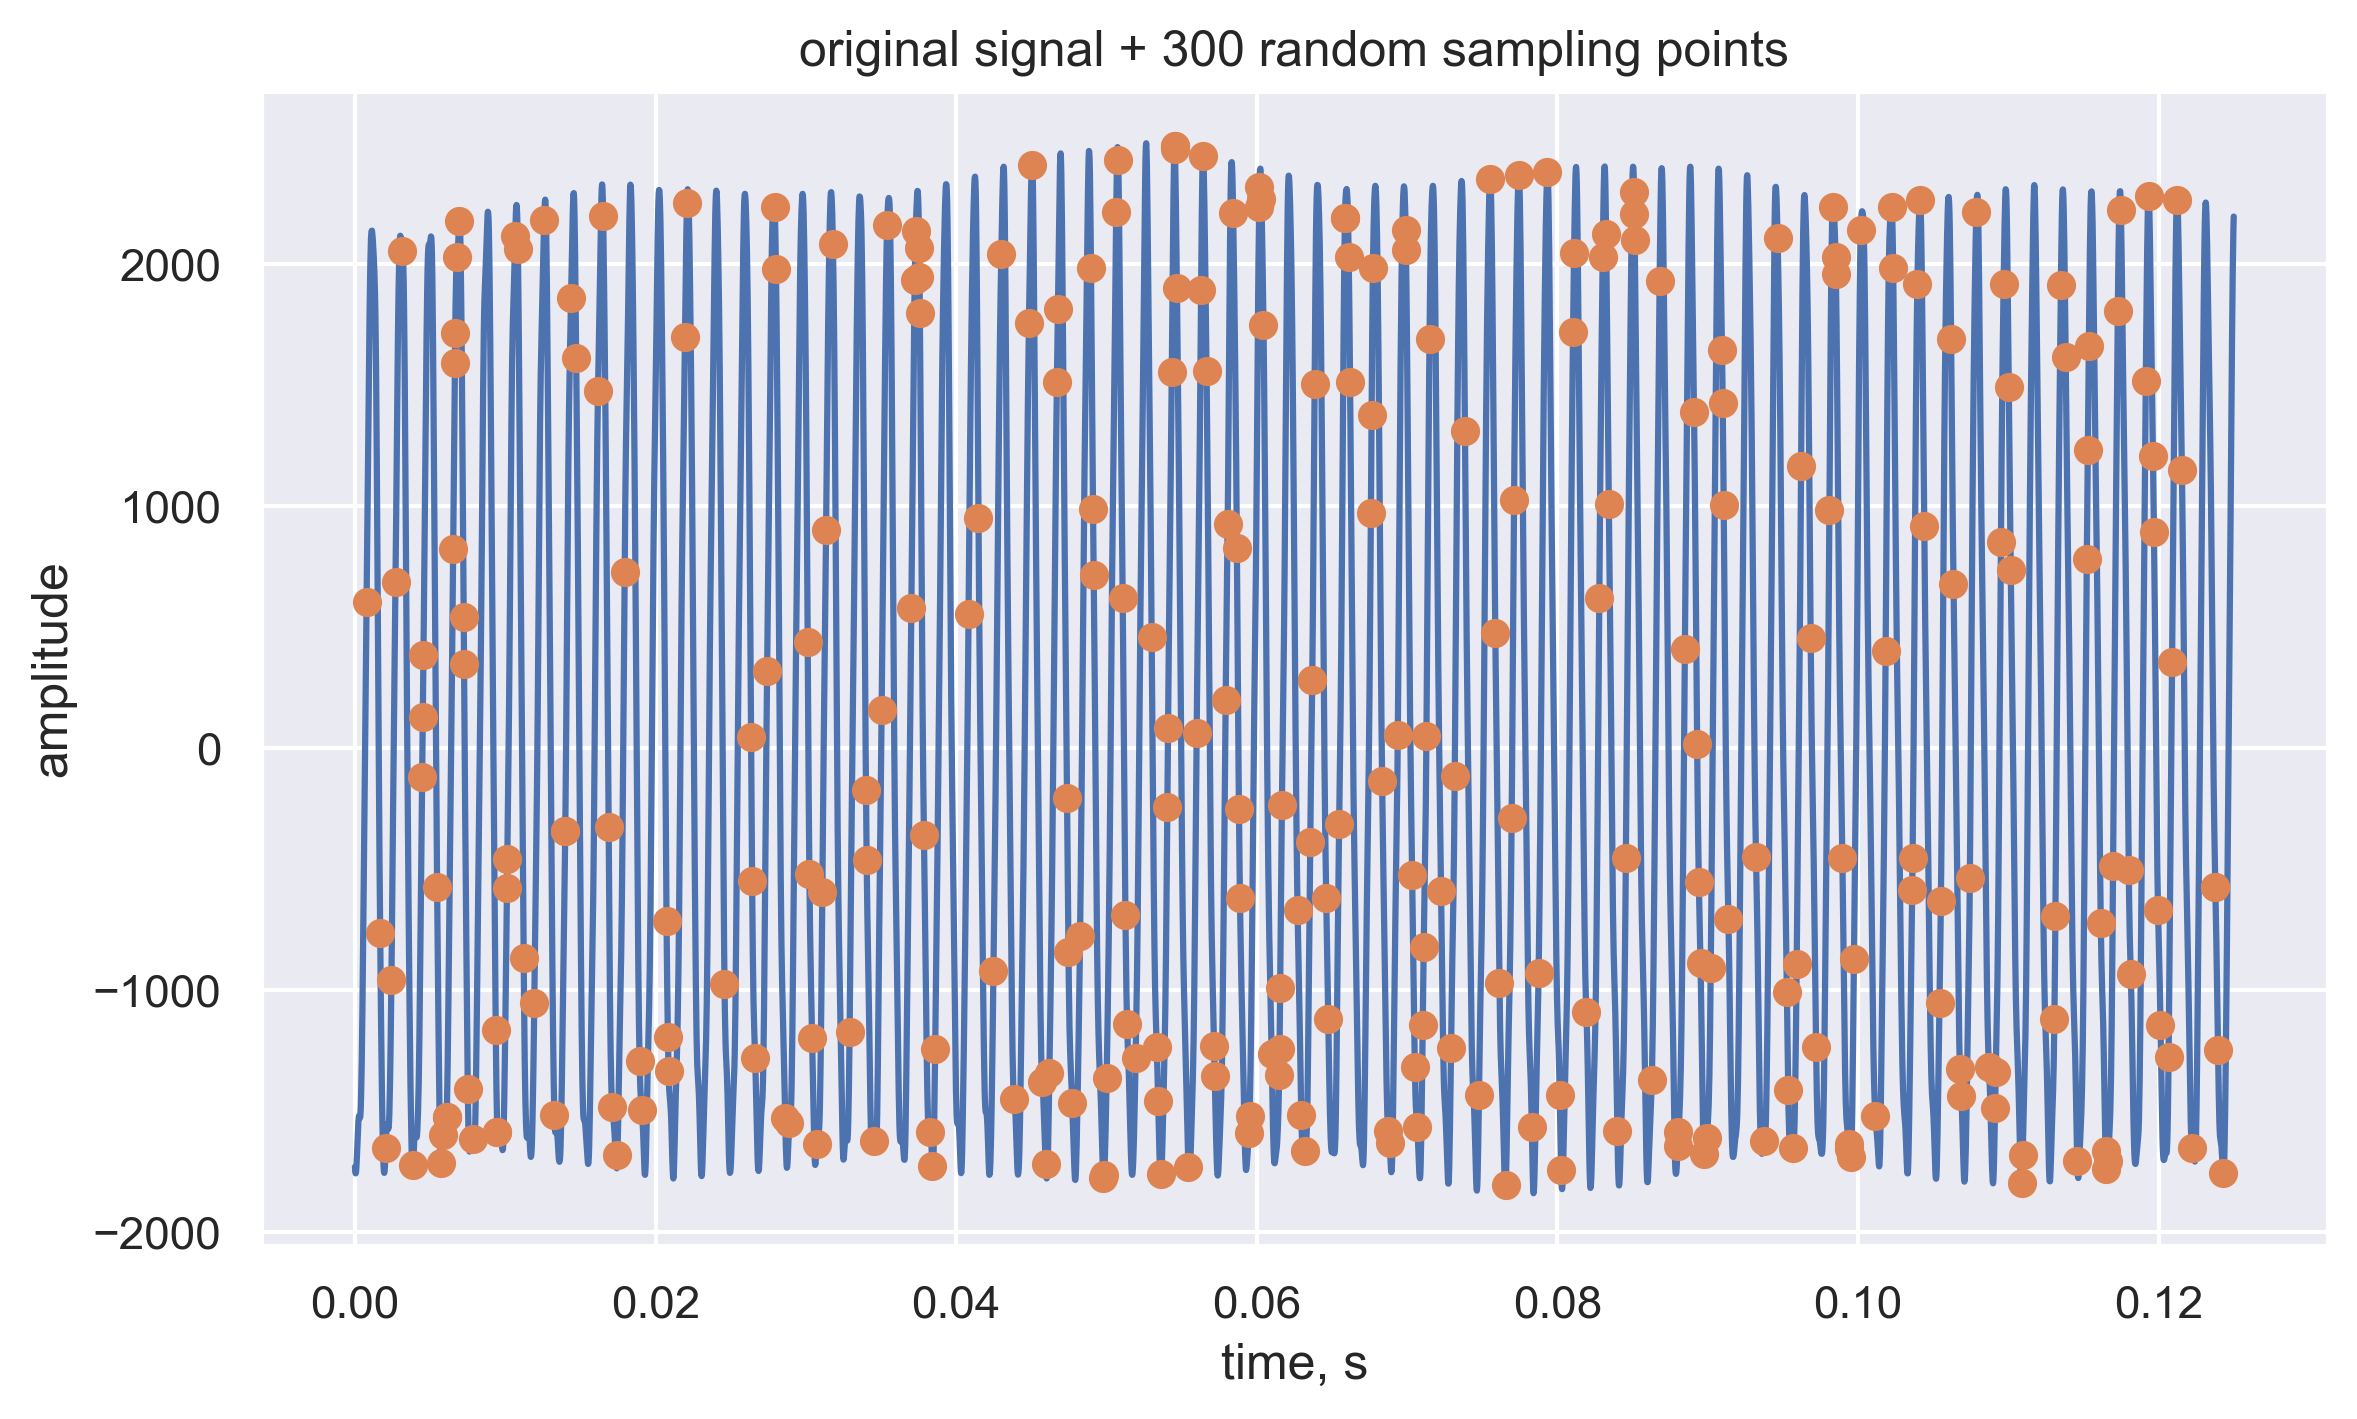
\includegraphics[width=\textwidth]{random_sampling.png}
	\caption{Original synthesized C$_5$ piano note (blue) and random measurements (orange).}
	\label{fig:random-sampling}
\end{figure}

In this model, sampling points consist of a discrete set of indices containing the signal amplitude corresponding to an instantaneous point in time. The random measurements actually point to these indices, which subset the chosen sparsifying basis: in this case, the DCT domain, for simplicity. The same random indices are used to select the rows of the DCT matrix of shape $n \times n$, where $n$ is the signal dimension. I then stack these rows to form the sensing matrix $\vec{A}$; essentially a partial DCT matrix of shape $m \times n$, where $m$ is the number of random measurements. Essentially, I am simulating a sensing device that not only purposely undersamples, but also samples at random, intermittent points in time.

In Chapter \ref{chap:theory}, I discussed an overview of popular algorithms used in CS. For the purposes of comparison in this chapter, I will be focusing on a gradient-based method (LASSO), and a convex optimization-based method (CVXPY). The optimization objectives for these two become

\begin{align}
\mathrm{LASSO}:& \quad \min_{\bm\hat{\vec{x}}} \frac{1}{2m} \norm{\vec{y} - \vec{A}\bm\hat{\vec{x}}}_2^2 + \alpha \norm{\bm\hat{\vec{x}}}_1 \label{eq:random-lasso-objective} \\
\mathrm{CVXPY}:& \quad \min_{\bm\hat{\vec{x}}} \norm{\bm\hat{\vec{x}}}_1 \quad \textrm{subject to} \quad \vec{A}\bm\hat{\vec{x}} = \vec{y} \label{eq:random-cvxpy-objective}
\end{align}

\noindent where $\bm\hat{\vec{x}}$ is the candidate solution, and the optimum value of $\alpha$ is automatically determined via 10-fold cross validation. A detailed implementation is shown in Appendix \ref{appendix:codes}. Figure~\ref{fig:random-compare-algorithms} shows a comparison of the original signal with the reconstructions from the two algorithms in the time and frequency domains. In the time domain, both algorithms appear to have been able to successfully reconstruct the signal, though the CVXPY recovery shows many artifacts. The LASSO algorithm yields a mean-squared error (MSE) of 0.002, while CVXPY yields an MSE of 0.074. In the frequency domain, however, many frequencies are erroneously being recovered by the LASSO method, and more so with the CVXPY method. Because LASSO's $\alpha$ is a hyperparameter, it will need additional tuning to yield a more optimal value.

\begin{figure}[htb]
	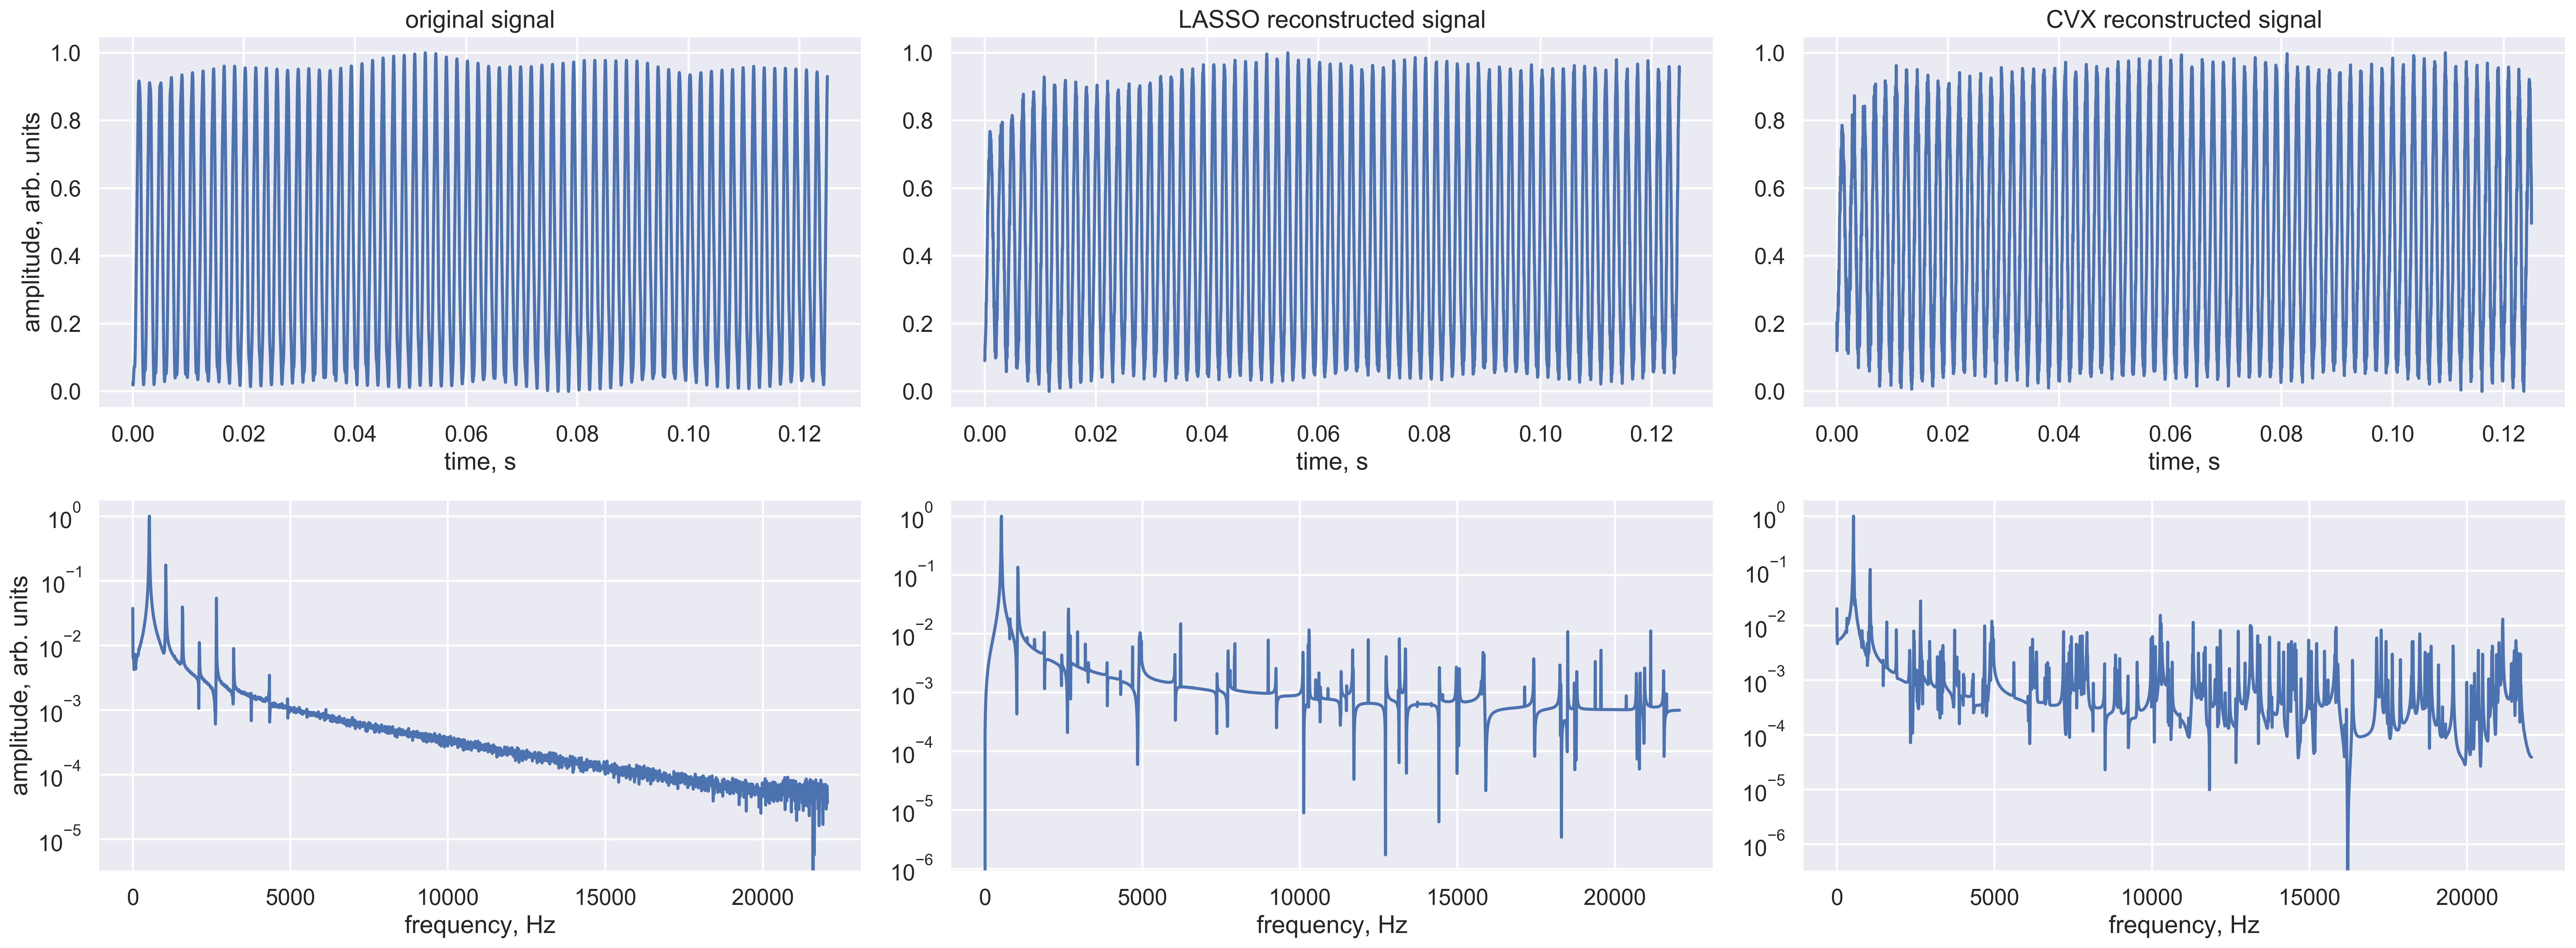
\includegraphics[width=\textwidth]{reconstruction_methods.png}
	\caption{Original signal (left column), LASSO reconstruction (middle column), and CVXPY reconstruction (right column). The top row shows the time domain representation, while the bottom row shows the frequency domain representation.}
	\label{fig:random-compare-algorithms}
\end{figure}


\section{Effect of random distribution on reconstruction error}
\label{sec:random-distro}
So far, I have worked solely with uniformly-distributed random sampling. Here, I investigate and compare the quality of reconstruction (in MSE) in terms of the random distribution. I will be working with two common distributions: the Gaussian and Poisson distributions, as well as the triangular distribution, which is commonly used in audio and image dithering. For each distribution, I generate i.i.d.~random variables and use these to compressively sample the signal. I then evaluate the reconstruction MSE and take the average over 10 iterations to obtain error bars.

\subsection{Uniform}
\label{ssec:random-distro-uniform}
The uniform distribution is given by

\begin{equation}
\label{eq:random-uniform}
U(x) = \begin{cases}
\frac{1}{b - a} & a \leq x \leq b, \\
0 & \mathrm{otherwise}
\end{cases}
\end{equation}

\noindent where $a$ and $b$ are the lower and upper bounds, respectively.

\subsection{Gaussian}
\label{ssec:random-distro-gaussian}
The Gaussian/normal distribution can be generated by

\begin{equation}
\label{eq:random-gaussian}
G(x) = \frac{1}{\sqrt{2\pi\sigma^2}} \exp[-\frac{(x - \mu)^2}{2\sigma^2}]
\end{equation}

\noindent where the parameters $\mu: \mu \in \mathbb{R}$ \& $\sigma^2: \sigma > 0$ are the distribution's mean and variance, respectively.

\subsection{Poisson}
\label{ssec:random-distro-poisson}
The Poisson distribution can be generated by

\begin{equation}
\label{eq:random-poisson}
P(x) = \frac{\lambda^x e^{-\lambda}}{x!}
\end{equation}

\noindent where the parameter $\lambda: \lambda > 0$ is the distribution's mean and variance.

\subsection{Triangular}
\label{ssec:random-distro-triangular}
The triangular distribution is generated by

\begin{equation}
\label{eq:random-triangular}
T(x) = \begin{cases}
0 & x < a, \\
\frac{2(x-a)}{(b - a)(c - a)} & a \leq x < c, \\
\frac{2}{b - a} & x = c, \\
\frac{2(b - x)}{(b - a)(b - c)} & c < x \leq b, \\
0 & x > b
\end{cases}
\end{equation}

\noindent where $a: a \in (-\infty, +\infty)$ is the lower bound, $b: b > a$ is the upper bound, and $c: a \leq c \leq b$ is the mode.

\subsection{Results \& discussion}
\label{ssec:random-distro-rnd}
Due to the computational requirements, I will only work with the first 1/32 seconds of the signal, corresponding to 1378 samples. Figure~\ref{fig:random-pdf} shows the probability density for each distribution.

\begin{figure}[htb]
	\centering
	\begin{subfigure}[h!]{0.49\textwidth}
		\centering
		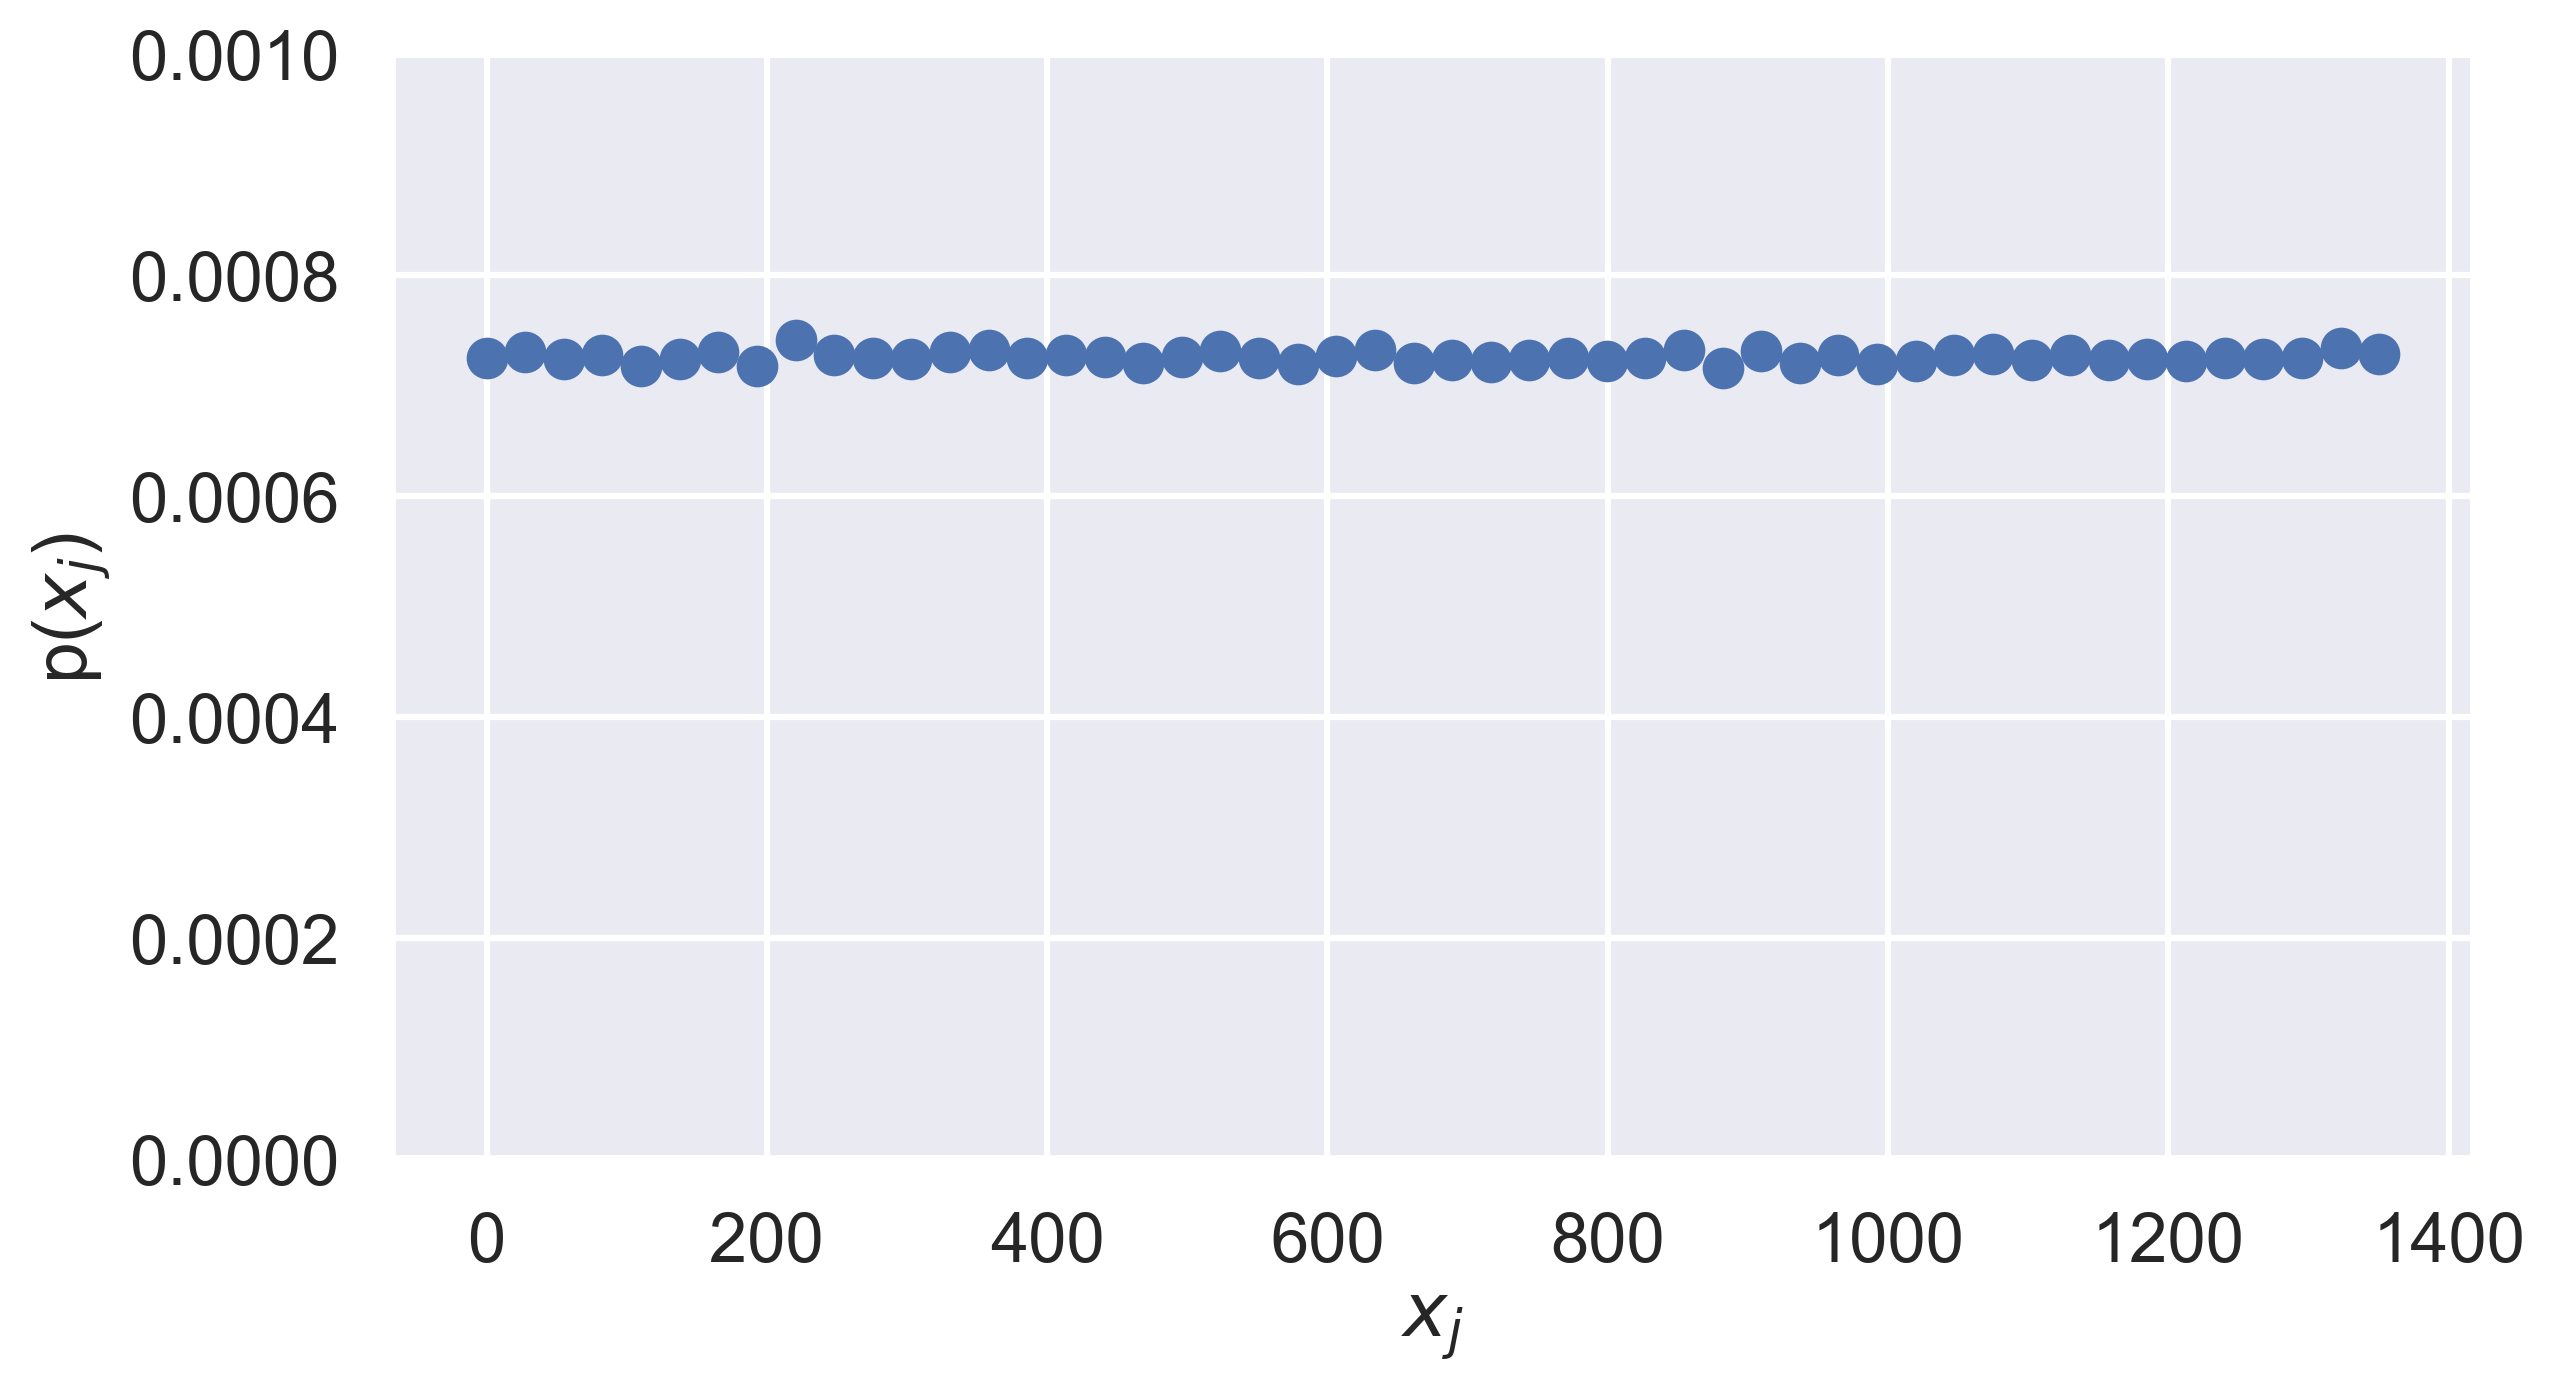
\includegraphics[width=\textwidth]{uniform_random.png}
		\caption{Uniform}
		\label{fig:random-pdf-uniform}
	\end{subfigure}
	\begin{subfigure}[h!]{0.49\textwidth}
		\centering
		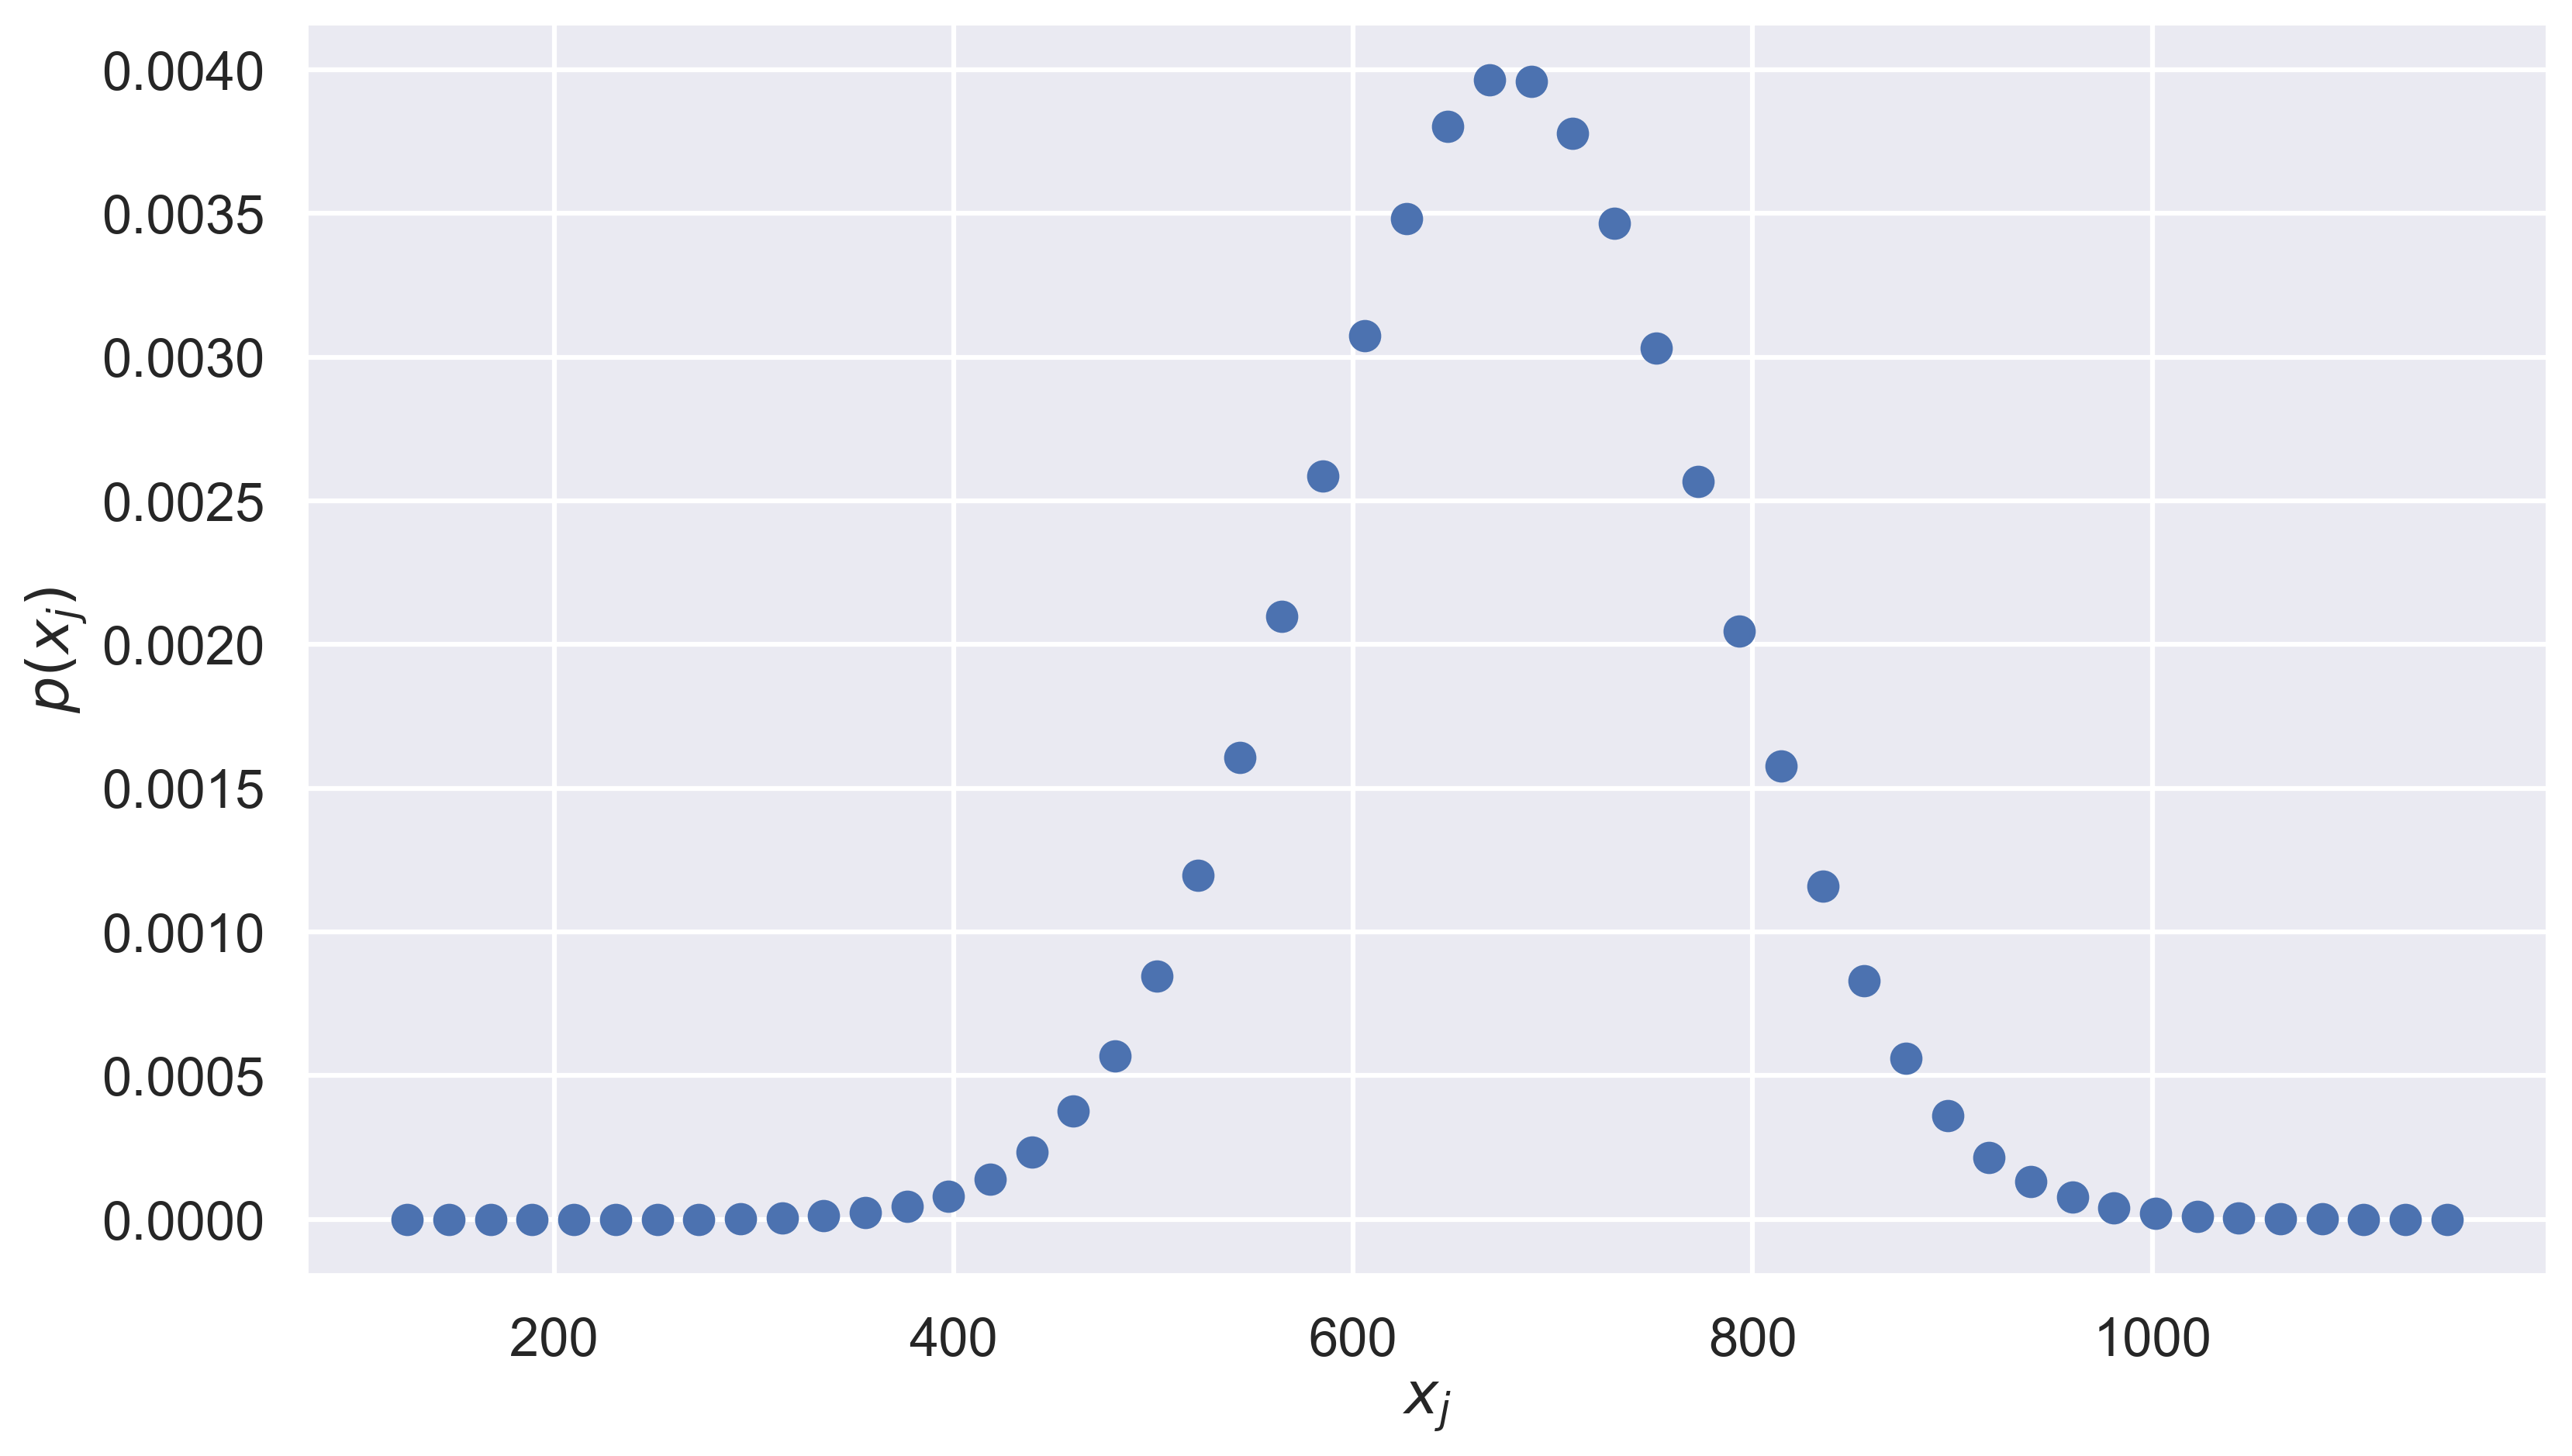
\includegraphics[width=\textwidth]{gaussian_random.png}
		\caption{Gaussian ($\mu = n/2$, $\sigma = 100$)}
		\label{fig:random-pdf-gaussian}
	\end{subfigure}
	\begin{subfigure}[h!]{0.49\textwidth}
		\centering
		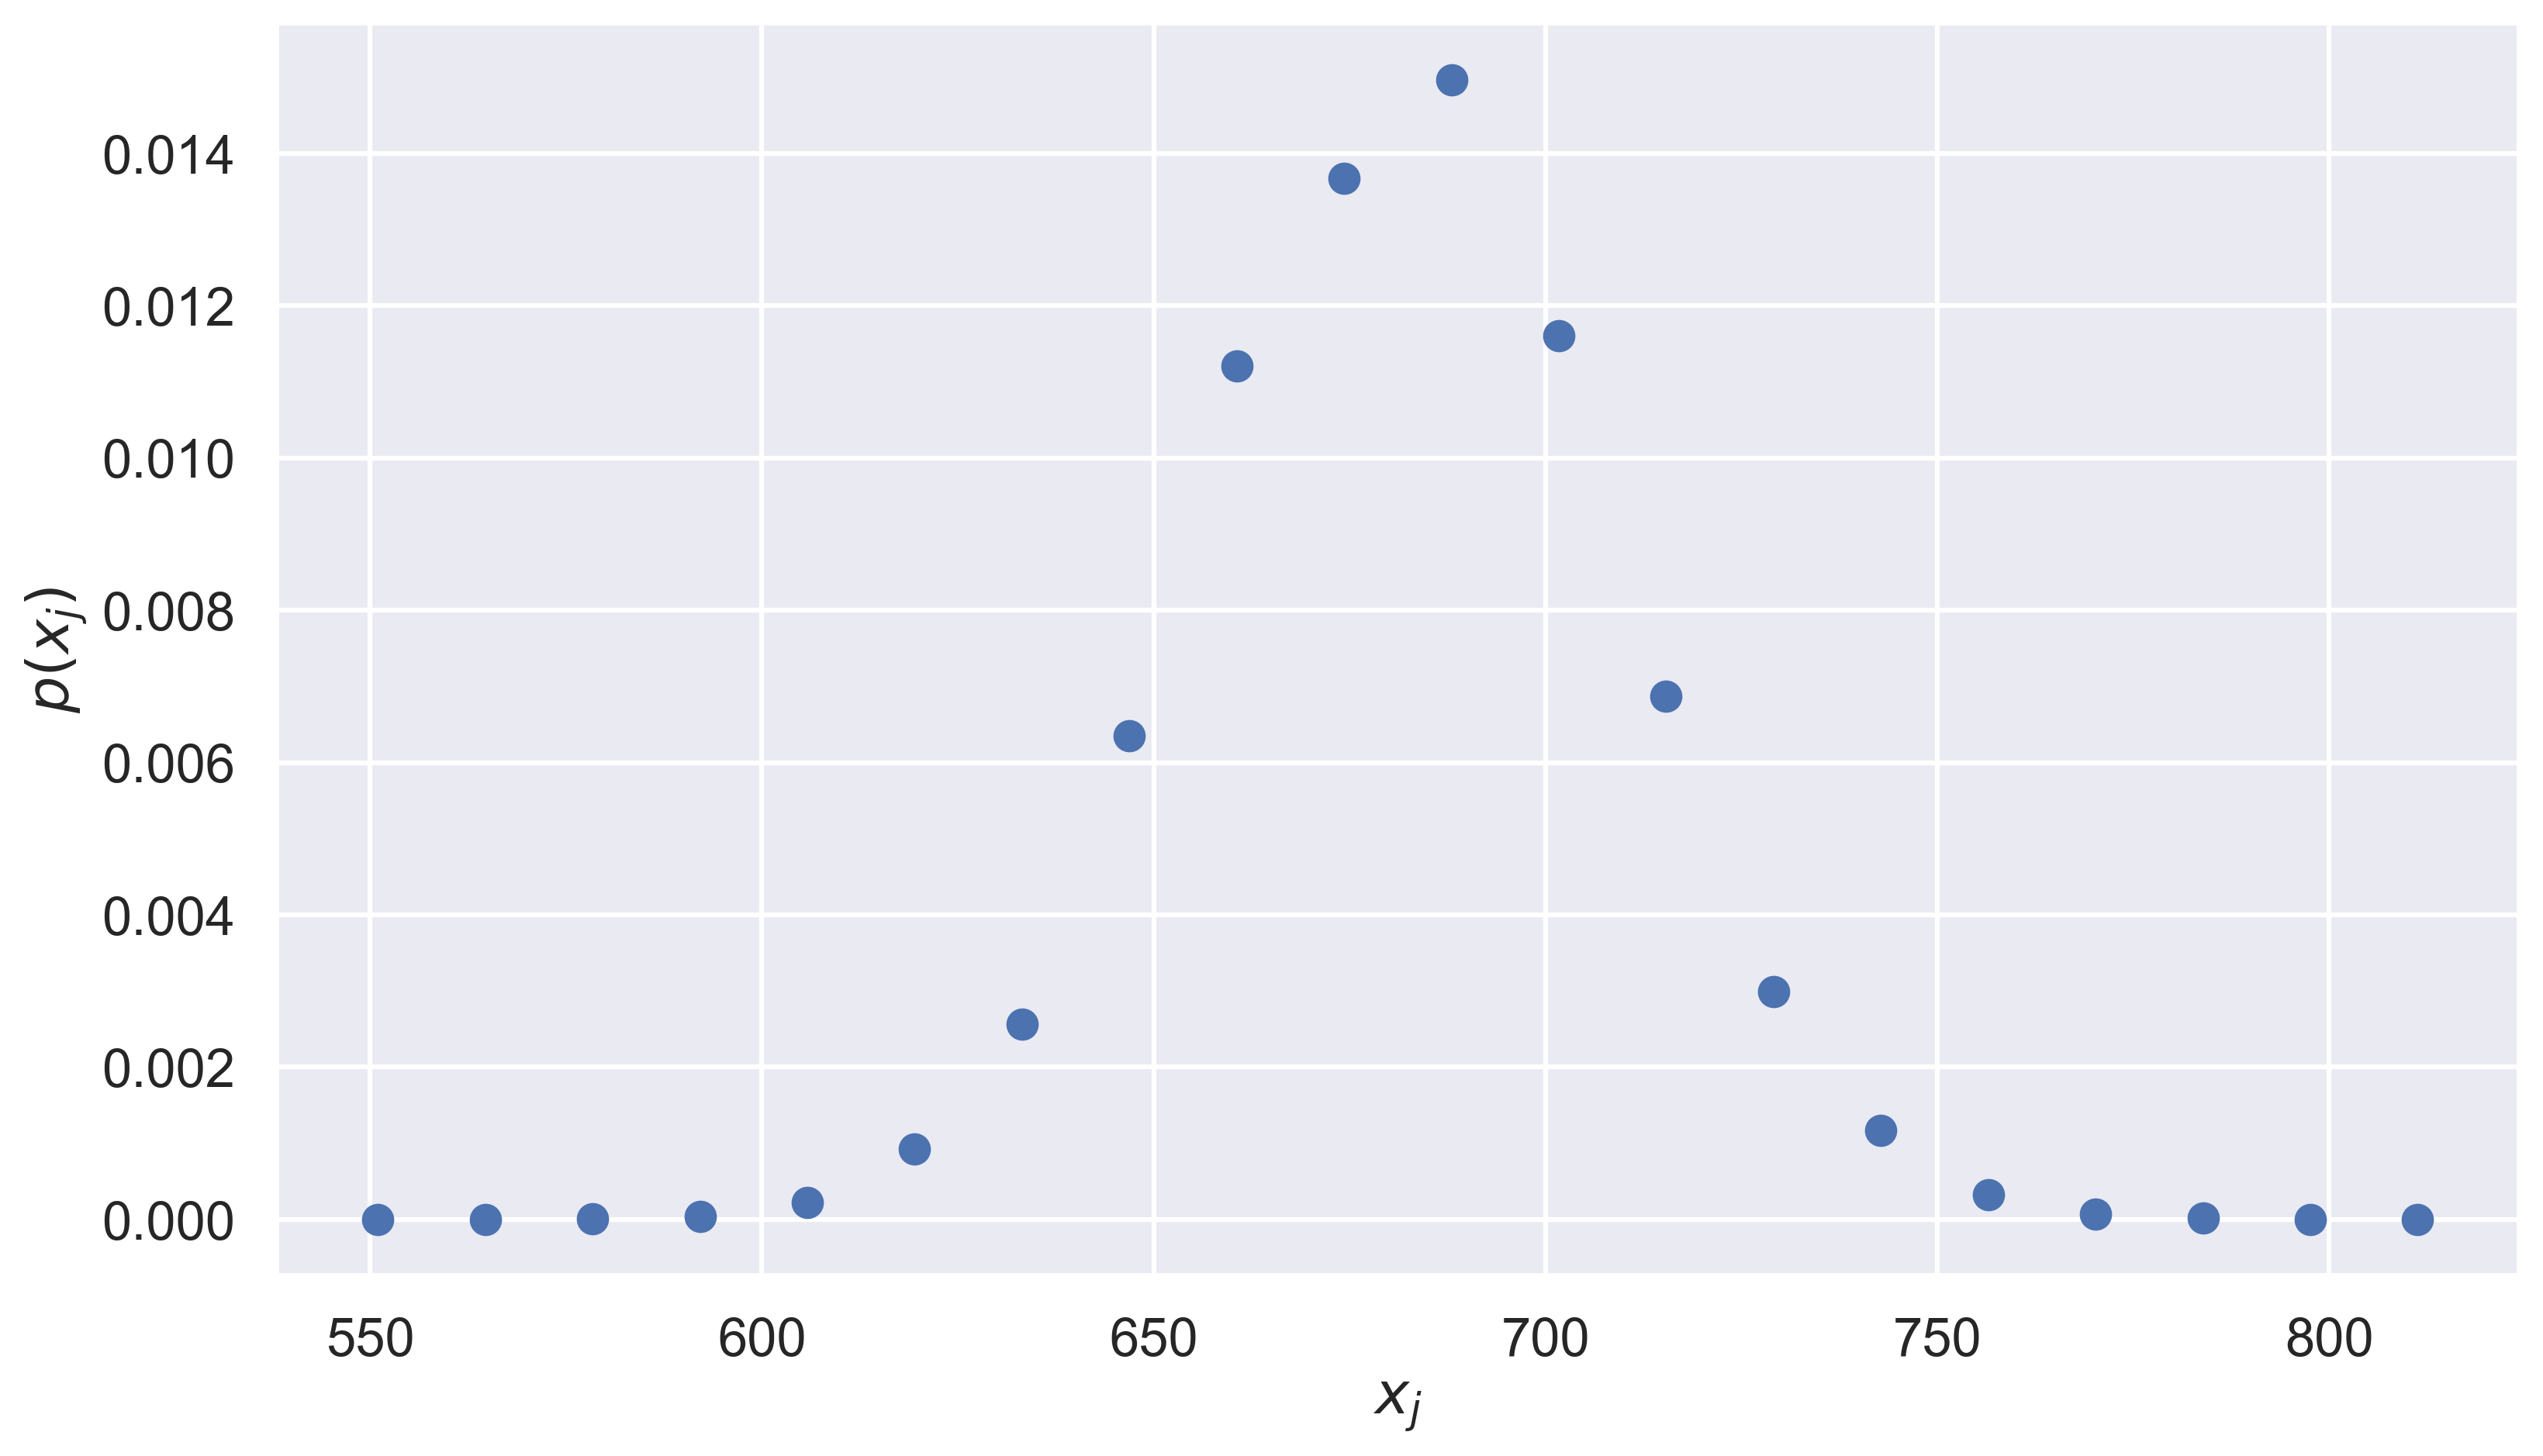
\includegraphics[width=\textwidth]{poisson_random.png}
		\caption{Poisson ($\lambda = n/2$)}
		\label{fig:random-pdf-poisson}
	\end{subfigure}
	\begin{subfigure}[h!]{0.49\textwidth}
		\centering
		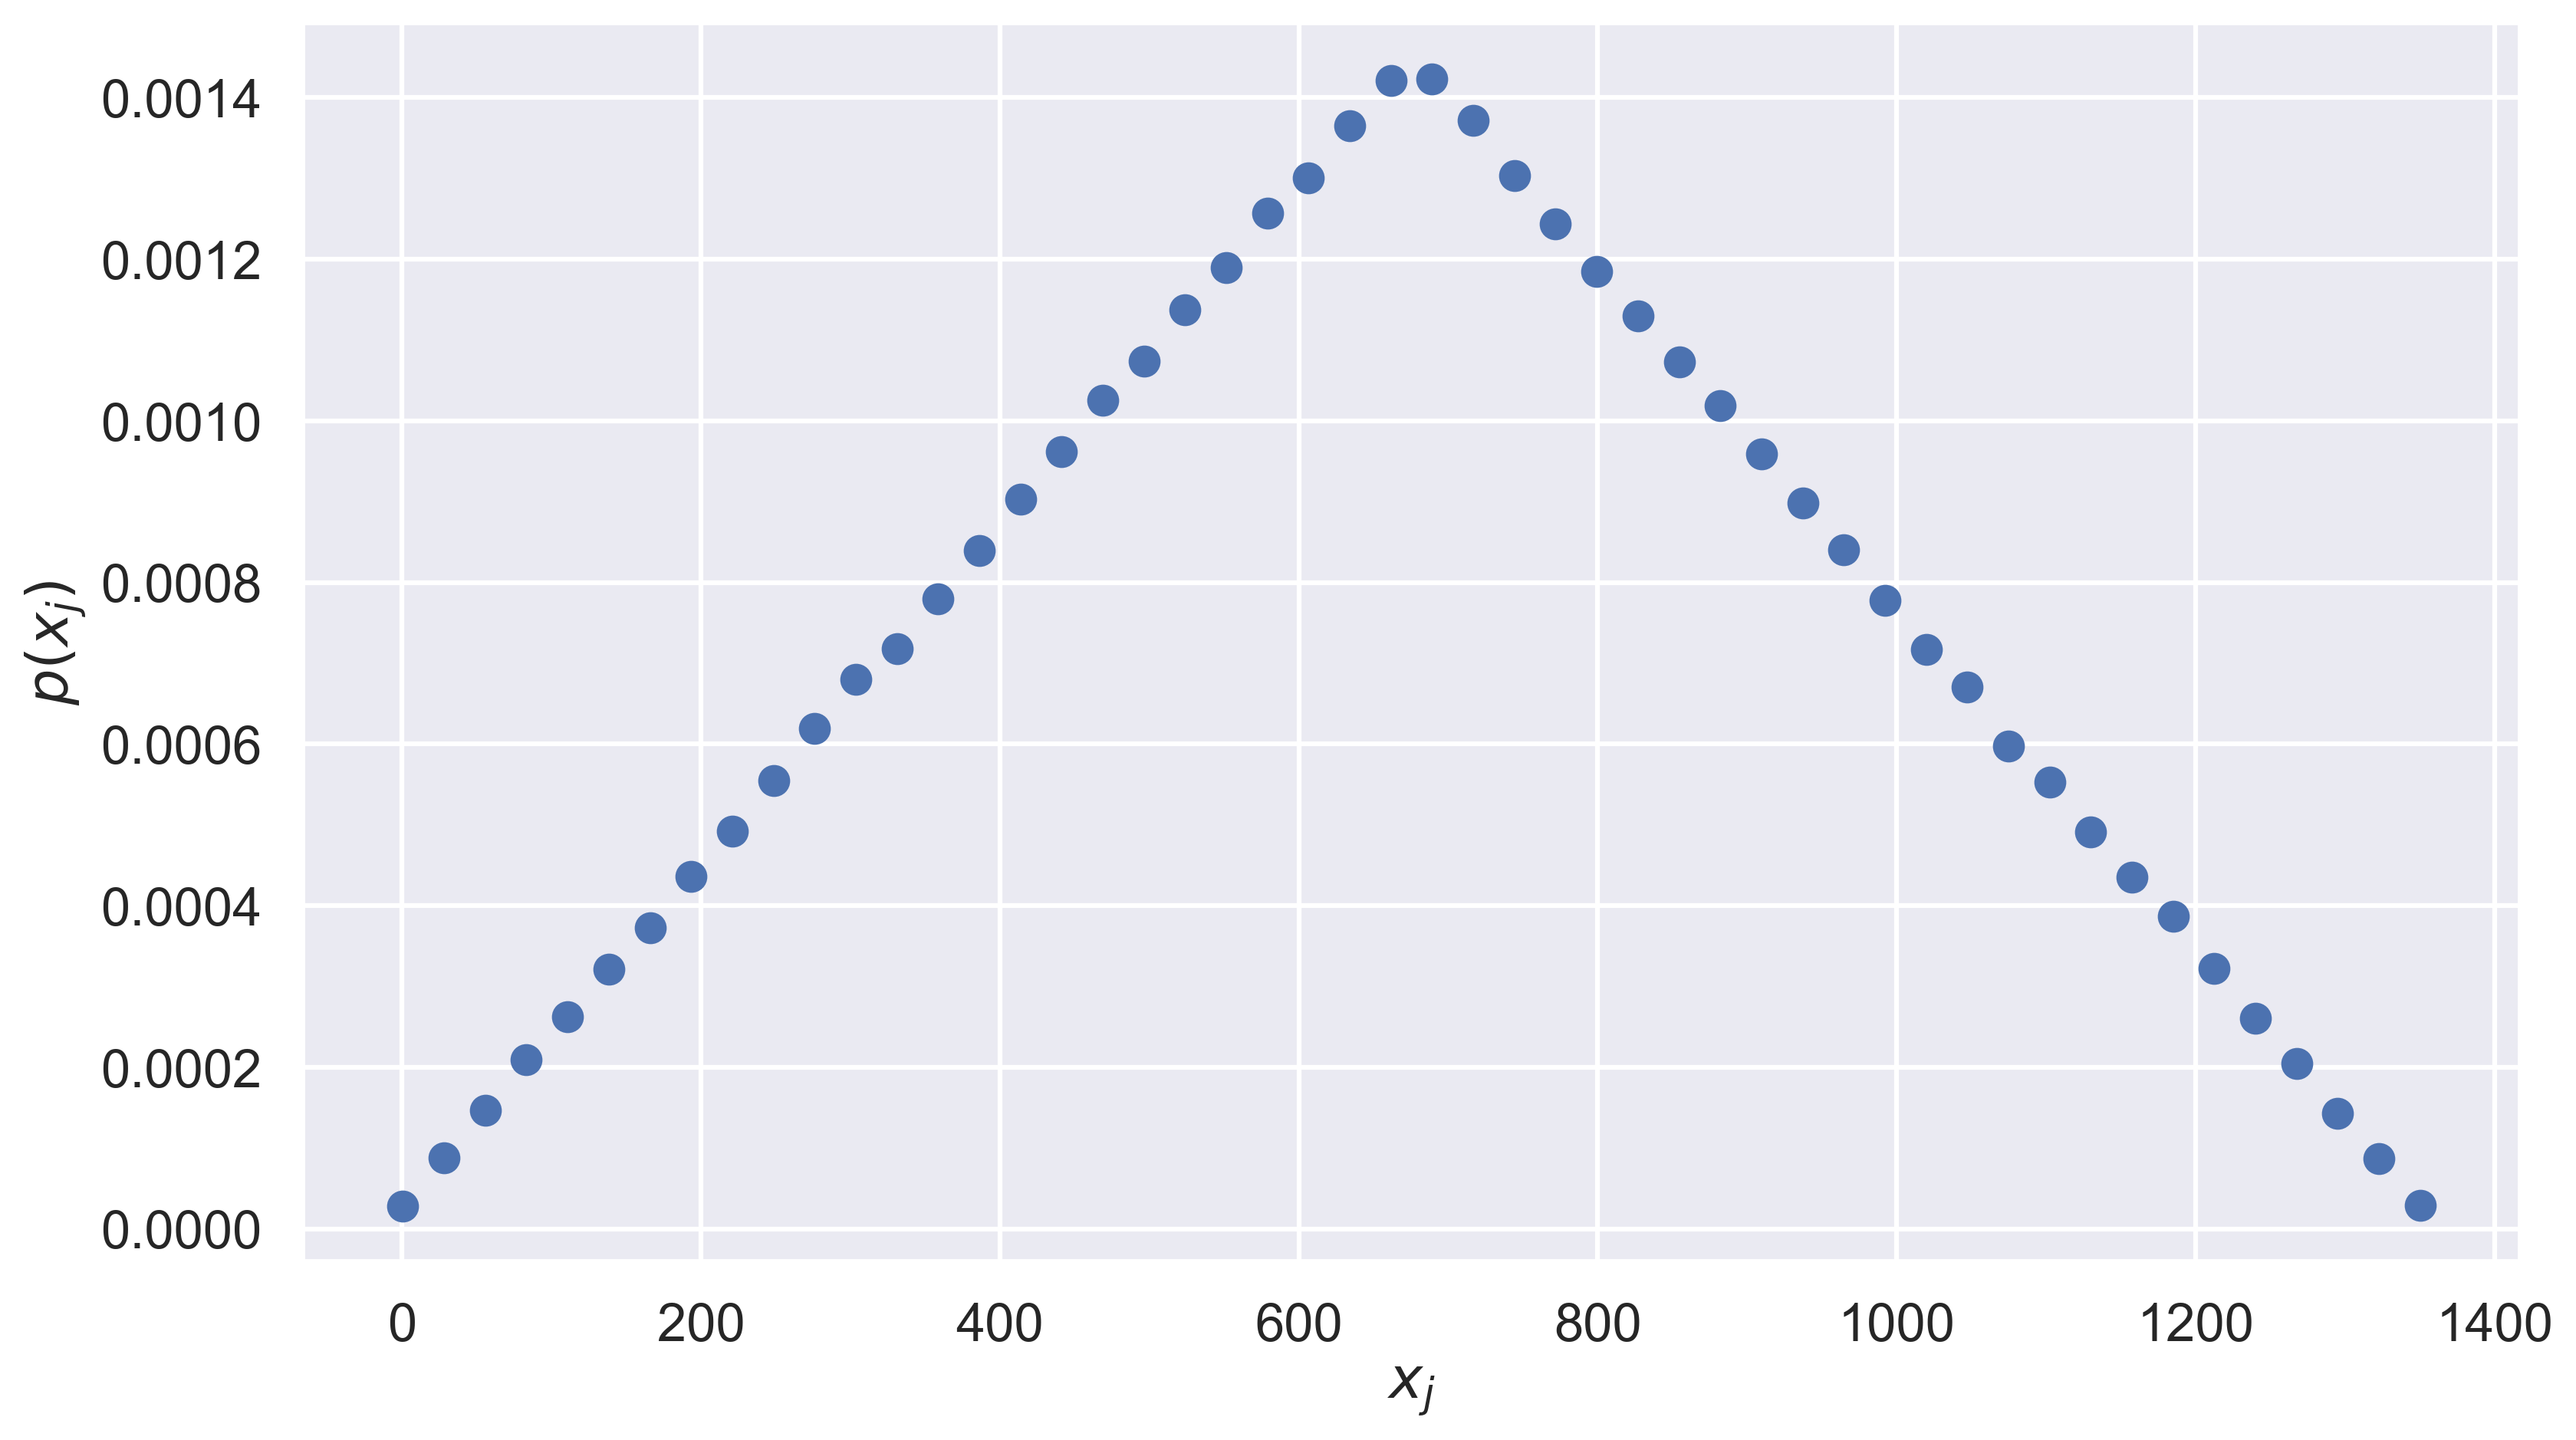
\includegraphics[width=\textwidth]{triangular_random.png}
		\caption{Triangular ($a = 0$, $b = n/2$, $c = n$)}
		\label{fig:random-pdf-triangular}
	\end{subfigure}
	\caption{Probability densities of the different random distributions used in this section, corresponding to the signal indices.}
	\label{fig:random-pdf}
\end{figure}

Figure~\ref{fig:random-mse} shows the MSE evaluated for each random distribution as a function of the fraction of total samples, more aptly referred to as the compression ratio. From this, we can observe that the uniform and triangular distributions give the lowest reconstruction error, but the latter has a more consistent performance across a wide range of compression ratios. They are followed, in order, by the Poisson and Gaussian distributions. One reason for the former's performance is that they are able to completely span the signal with appreciable probability near the bounds, while the latter's probability near the bounds are quickly approaching zero.

\begin{figure}[htb]
	\centering
	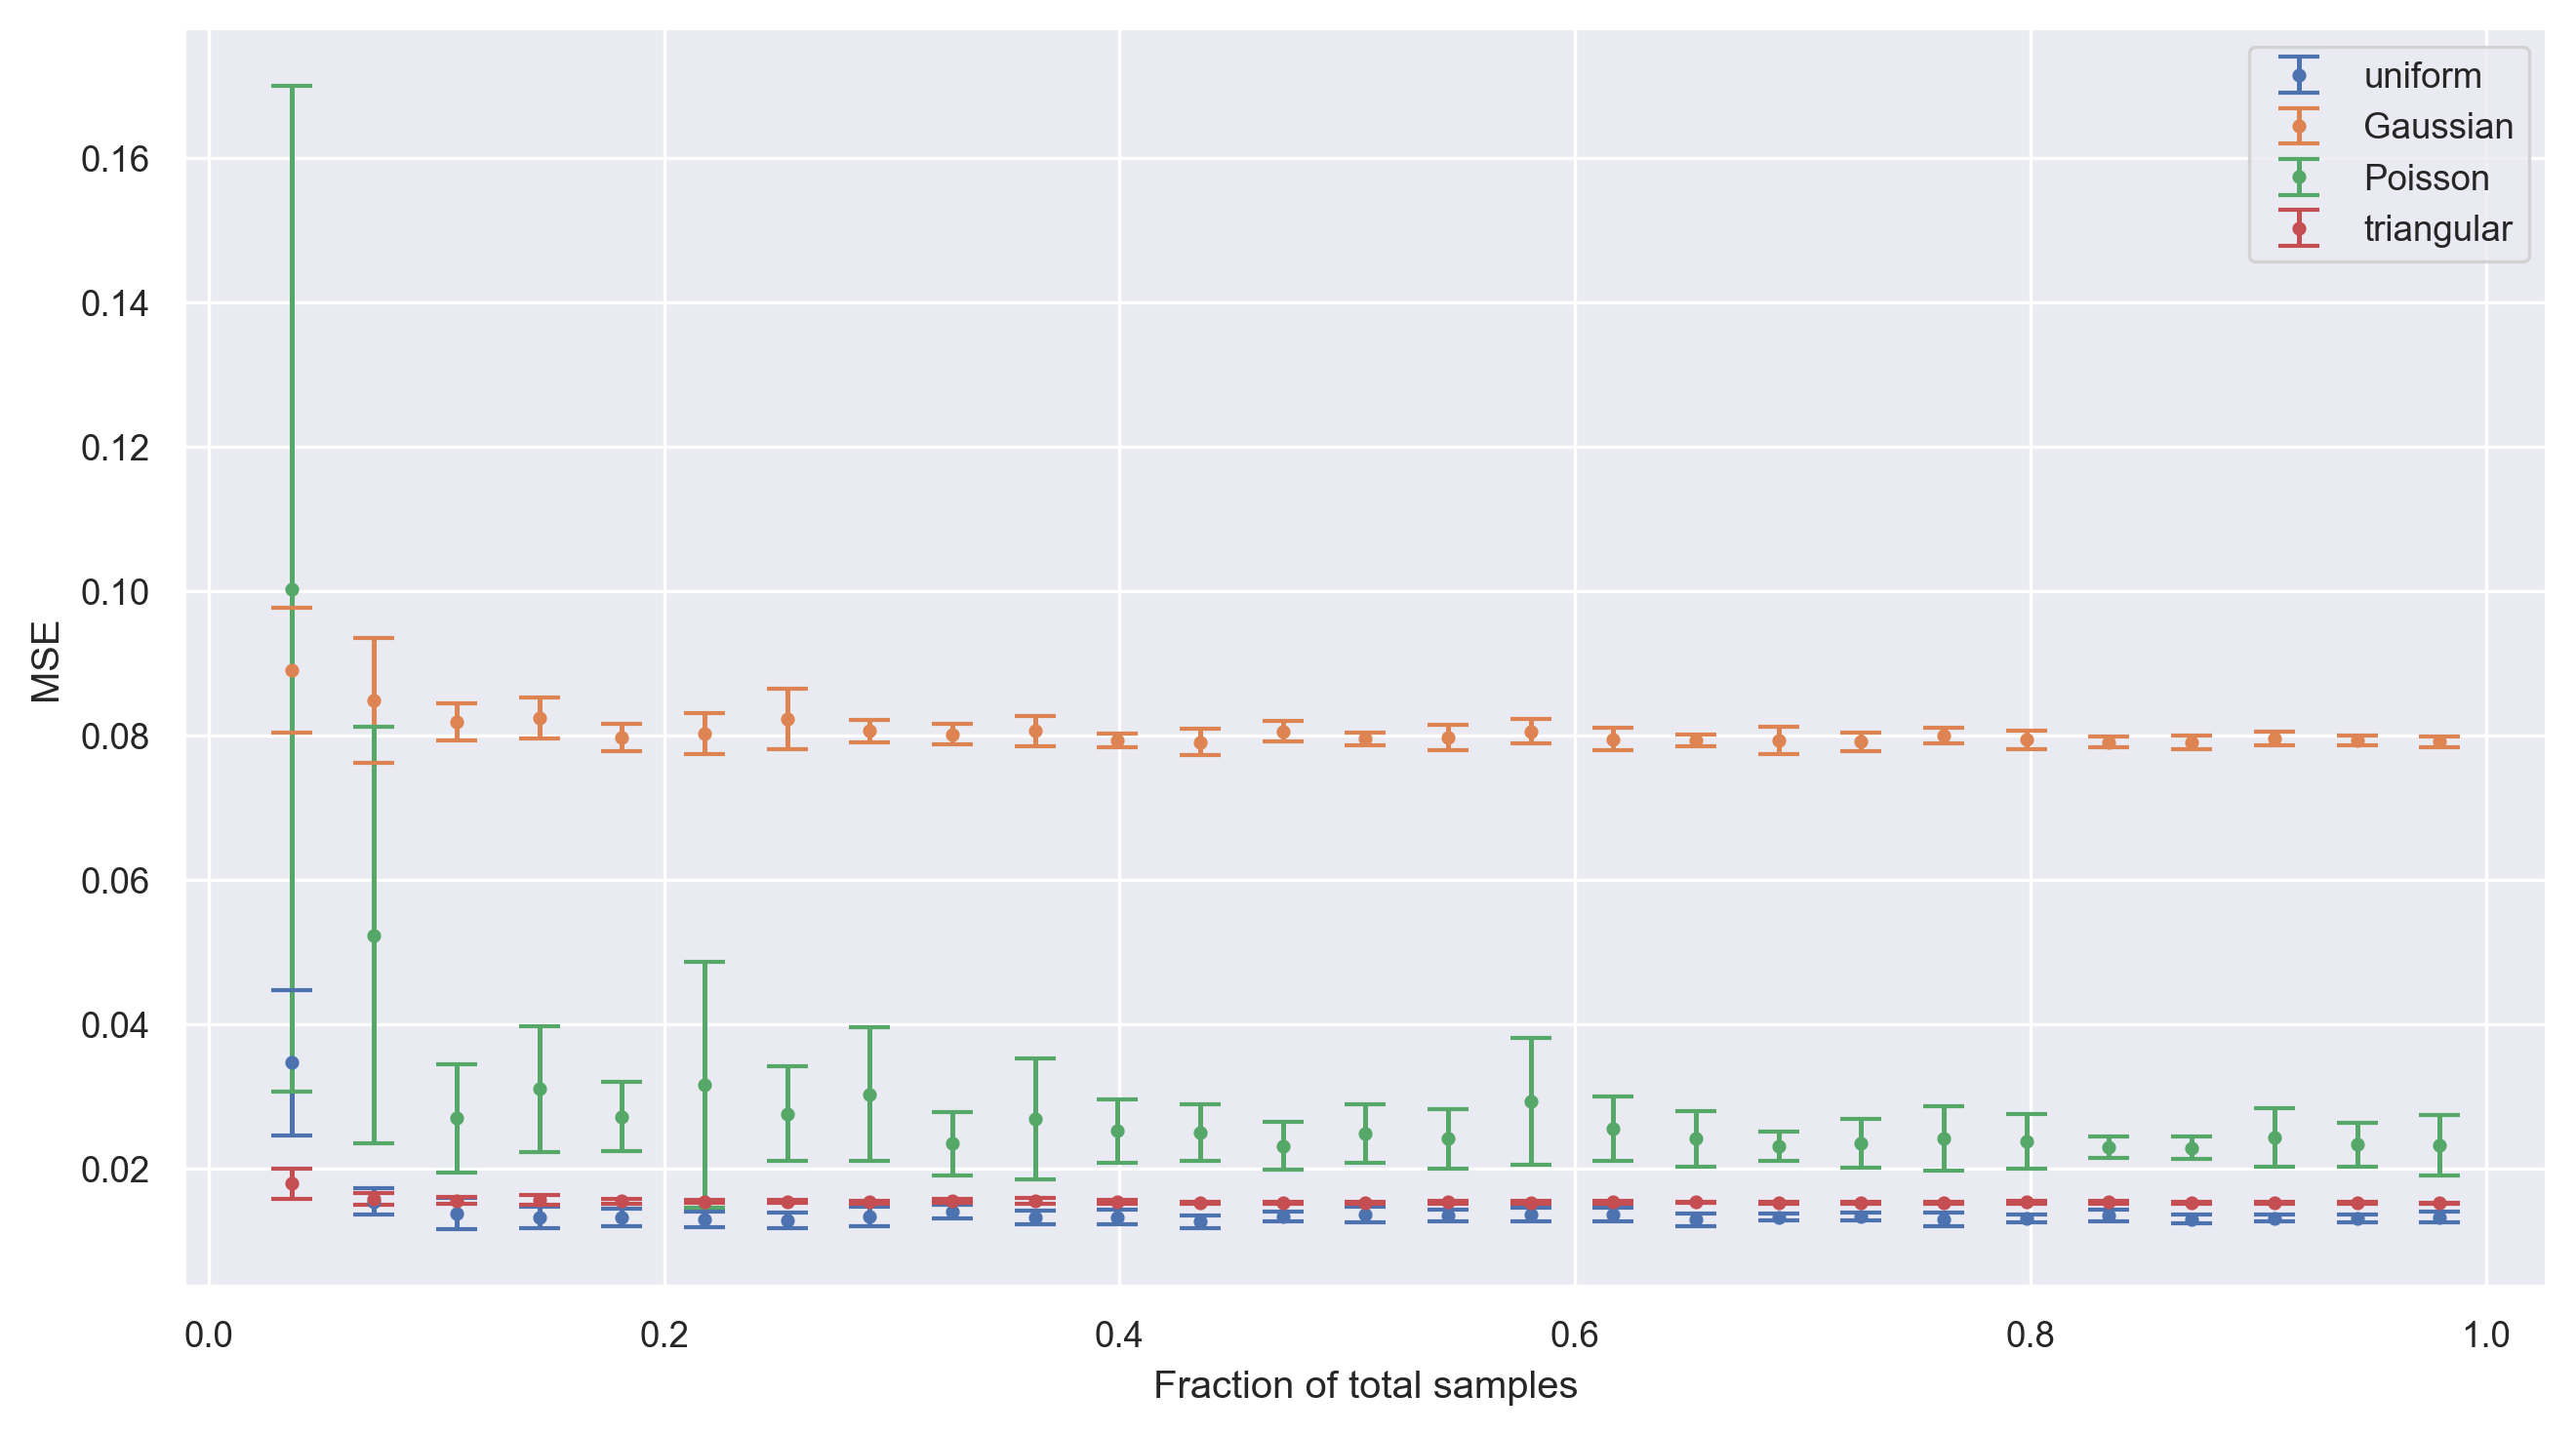
\includegraphics[width=\textwidth]{random_mse.png}
	\caption{Evaluated MSE for each random distribution as a function of compression ratio, average over 10 iterations.}
	\label{fig:random-mse}
\end{figure}

In line with these findings, I will be using uniformly-distributed random variables throughout this study unless otherwise stated. In a later chapters, I will be exploring more on recovering exact frequencies and their harmonics beyond the Nyquist rate in real signals, as well as signals with multiple frequencies.